\documentclass[tikz,border=10pt]{standalone}
\usepackage{tikz}

\begin{document}

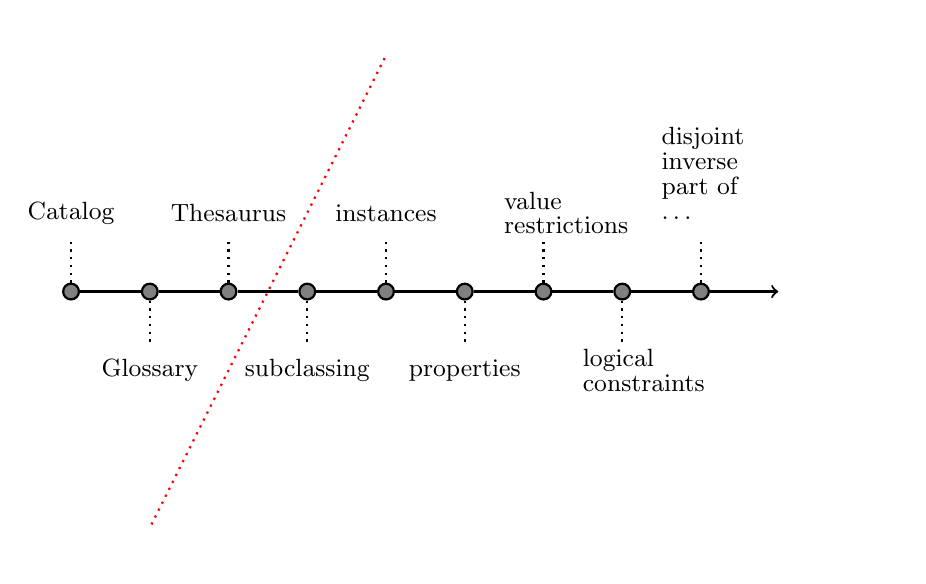
\begin{tikzpicture}

\tikzstyle{dummy} = [rectangle,minimum height=2em, inner sep=0pt, outer sep=0pt,font=\fontsize{9}{9}\selectfont];%
\tikzstyle{circ} = [circle,draw=black, minimum height=1em, text centered, fill=black!50,thick,inner sep=0pt,minimum size=2mm];

\node[circ] at (0,0) (1) {} ; 
\node[dummy] at (0,1) (d1) {Catalog};
\path (1) edge[-,thick,dotted] (d1);

\node[circ] at (1,0) (2) {} ; 
\node[dummy] at (1,-1) (d2) {Glossary};
\path (2) edge[-,thick,dotted] (d2);

\node[circ] at (2,0) (3) {};
\node[dummy] at (2,1) (d3) {Thesaurus};
\path (3) edge[-,thick,dotted] (d3);

\node[circ] at (3,0) (4) {} ; 
\node[dummy] at (3,-1) (d4) {subclassing}; %
\path (4) edge[-,thick,dotted] (d4);

\node[circ] at (4,0) (5) {} ; 
\node[dummy] at (4,1) (d5) {instances};
\path (5) edge[-,thick,dotted] (d5);

\node[circ] at (5,0) (6) {} ; 
\node[dummy] at (5,-1) (d6) {properties};
\path (6) edge[-,thick,dotted] (d6);

\node[circ] at (6,0) (7) {} ; 
\node[dummy] at (6,1) (d7) {};
\node[dummy] at (7,1) (d7a) {\parbox[r][2cm][c]{3cm}{value\\ restrictions}};
\path (7) edge[-,thick,dotted] (d7);

\node[circ] at (7,0) (8) {} ; 
\node[dummy] at (7,-1) (d8) {};
\node[dummy] at (8,-1) (d8a) {\parbox[r][2cm][c]{3cm}{logical\\ constraints}};
\path (8) edge[-,thick,dotted] (d8);

\node[circ] at (8,0) (9) {} ; 
\node[dummy] at (8,1) (d9) {};
\node[dummy] at (9,1.5) (d9a) {\parbox[r][2cm][c]{3cm}{disjoint\\ inverse \\ part of \\ $\dots$}};
\path (9) edge[-,thick,dotted] (d9);

\path (1) edge[-,thick] (2) ;
\path (2) edge[-,thick] (3) ;
\path (3) edge[-,thick] (4) ;
\path (4) edge[-,thick] (5) ;
\path (5) edge[-,thick] (6) ;
\path (6) edge[-,thick] (7) ;
\path (7) edge[-,thick] (8) ;
\path (8) edge[-,thick] (9) ;
\node[dummy] at (9,0) (d10) {};
\path (9) edge[->,thick] (d10);

\node[dummy]  at (4,3) (c1) {};
\node[dummy]  at (1,-3) (c2) {};
\path (c1) edge[-,thick,dotted,color=red] (c2);

\end{tikzpicture}

\end{document}